The doubly linked list is the same than singly linked list but as the name tell us we have another pointer to the previous element, something like this:

\begin{figure}[H]
    \centering
    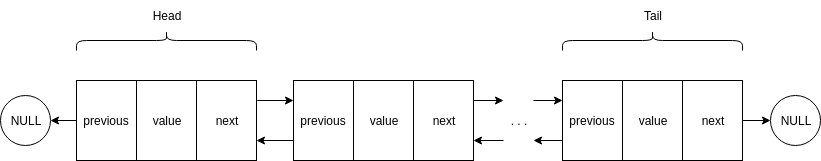
\includegraphics[width=1.00\textwidth]{Images/DataStructures/LinkedLists/DoublyLinkedList.png}
    \caption{Diagram of a doubly linked list}
    \label{fig:doubly_linked_list_diagram-01}
\end{figure}

And here you are my own implementation of this data structure, you can nottice that is very similar to a singly linked list:

\begin{lstlisting} 
    #include <bits/stdc++.h>

    using namespace std;

    struct Node{

        Node *previous;
        Node *next;
        int value;

        Node(int _value){
            previous = next = NULL;
            value = _value;
        }

    };

    struct LinkedList{

        int size;
        Node *head;
        Node *tail;

        LinkedList(){
            size = 0;
            head = tail = NULL;
        }

        void InsertAtTail(int value){
            Node *node = new Node( value );
            if(size == 0)
                head = tail = node;
            else {
                tail -> next = node;
                node -> previous = tail;
                tail = node;
            }
            size++;
        }

        void InsertAtHead(int value){
            Node *node = new Node( value );
            if(size == 0)
                head = tail = node;
            else {
                node -> next = head;
                head -> previous = node;
                head = node;
            }
            size++;
        }

        void Delete(int index){
            Node *aux = head;
            if( index < size && index >= 0){
                int middle = size >> 1;
                for(int i = 0; i < index; i++)
                    aux = aux -> next;
                
                if(index == 0){
                    head = head -> next;
                    head -> previous = NULL;
                } else if ( index == size - 1){
                    tail = tail -> previous;
                    tail -> next = NULL;
                } else {    
                    aux -> previous -> next = aux -> next;
                    aux -> next -> previous = aux -> previous;
                    aux = NULL;
                }
            } else {
                cout << "\nInvalid index" << endl;
                return;
            }
            size--;
        }

        void DeleteAtHead(){
            head = head -> next;
            head -> previous = NULL;
        }

        void DeleteAtTail(){
            tail = tail -> previous;
            tail -> next = NULL;
        }

        int Search(int index){
            Node *aux = head;
            if(index < size){
                
                for(int i = 0; i < index; i++)
                    aux = aux -> next;
                
                return aux -> value;
            } else {
                cout << "\nIndex doesn't exists\n";
            }

            return INT_MIN;
        }

        int getSize(){
            return size;
        }

        bool IsEmpty(){
            return ( size == 0 );
        }

        void print(){
            Node *aux = head;
            cout << endl;
            while( aux != NULL ){
                cout << aux -> value << " ";
                aux = aux -> next;
            }
            cout << endl;   
        }

    };
\end{lstlisting}